\documentclass[10pt,xcolor=x11names,compress, show notes]{beamer}% pour l'impression, tout n'apparait qu'une fois \documentclass[handout,12pt]{beamer}

%\usepackage[scaled]{helvet}
\usepackage[round]{natbib}
\usepackage[utf8x]{inputenc}
\usepackage[USenglish]{babel}
\usepackage{todonotes}
\usepackage{color}

\usepackage{changepage}
\usepackage{pifont} %pour les symbole sympa \ding{nb}

%%% Pour Tikz
\usepackage{tikz}
\usetikzlibrary{calc}
%\usetikzlibrary{arrows,shapes,trees,positioning}  

%%%pour les plots matlab en tikz
\usepackage{pgfplots} 
\pgfplotsset{compat=newest}

%%% Pour les maths
\usepackage{bm}
\usepackage{amsmath,mathtools}
\usefonttheme[onlymath]{serif}
\usepackage{cancel} %pour barrer des math

%%% Pour la mise en forme
\usepackage[export]{adjustbox}
\usepackage{subcaption}
\usepackage{wrapfig}
\usepackage{pdfpages}
\setbeamertemplate{navigation symbols}{} 
\usepackage{array}
%\usepackage{subfigure}
%\usepackage[]{geometry}
%\usepackage{palatino}
%\setbeamertemplate{caption}{\raggedright\insertcaption\par}
\usepackage{multicol}
\setlength{\columnsep}{0cm}
\usepackage[framemethod=TikZ]{mdframed}

%%% Theme
\def \pied {} %content if footline
\usetheme{Alice}


%\setbeamertemplate{footline}{test}


%\useoutertheme[subsection=false]{miniframes} %%pour avoir le défilement en en-tête des diapos par section
%\setbeamercolor*{lower separation line head}{bg=DeepSkyBlue4} 

% Customisation 
\setlength{\fboxrule}{0.2pt}
\newcommand{\tikzmark}[1]{\tikz[remember picture] \coordinate (#1) ++ (-3pt,6pt) {};}
\newcommand{\citeTransp}[1]{\color{fg!50} \citep{#1}}
\renewcommand\bibsection{\section[]{~}}
\usepackage{algorithm}
\usepackage{algorithmic}
\graphicspath{{images/}}

%% Autre

\definecolor{main}{rgb}{0 0.439  0.753} %bleu %0 112 192
\definecolor{rouge}{rgb}{1 0.270 0 } %255 69 0
\definecolor{jaune}{rgb}{1 0.745 0} %255 190 0
\definecolor{vert}{rgb}{0.573 0.792 0.209} %146 202 74

\newlength{\avion}
\setlength{\avion}{0.5\textwidth}

\newlength{\larg}	\setlength{\larg}{0.5cm}	
\newlength{\haut}	\setlength{\haut}{4\larg}

\newcommand{\diag}[1]{\lceil#1\rfloor}
\newcommand*\circled[1]{\tikz[baseline=(char.base)]{
            \node[shape=circle,draw,inner sep=2pt,color=main,fill=main!10, line width=1pt] (char) {#1};}}

%%% Page de titre
%======================
\author{\underline{A. {Dinsenmeyer}}$^{1,2}$, Q. {Leclère}$^1$, J. {Antoni}$^1$ et E. Julliard$^3$}
\institute{$^1$ Laboratoire Vibrations Acoustique\\ $^2$ Laboratoire de Mécanique des Fluides et d’Acoustique\\Lyon, France \\ $^3$ Airbus, Toulouse}
\title{Débruitage de la matrice interspectrale pour l'étude des sources aéroacoustiques}
\subtitle{}
\titlegraphic{ 
\includegraphics[height=1cm]{logo/LABEX_CELYA.jpg} \hfill
 	  
\includegraphics[trim={0 3cm 0 3cm},clip=true,height=1cm]{logo/logo_ADAPT.png} \hfill
 
\includegraphics[height=1cm]{logo/LVA_compact_couleur.jpg} \hfill
 
\includegraphics[height=1cm]{logo/logo_lmfa.pdf} \hfill  }
\date{\small \vfill JJCAB -- Novembre 2018}
\begin{document}

%%%		Title
%======================
\begin{frame}[plain,t]
	\maketitle	
\end{frame}

%%% Context
%======================
\section*{Contexte}
\begin{frame}[t]{\insertsectionhead}
	\noindent\begin{minipage}{\textwidth}
		\begin{itemize}
		        \item<1-> \textbf{Mesures bruitées} : Extérieur venté, soufflerie, milieu sous-marin, etc.
		        	\item<2-> \textbf{Contexte industriel} : design moteur et profil			
		        \item<3-> 2 types de fluctuations de pression : \\
			$ \left. \begin{array}{l} 
			\mbox{- les sources acoustiques (\textcolor{jaune}{signal})} \\                   
			\mbox{- la turbulence de l'écoulement (\textcolor{rouge}{bruit})}                      
			\end{array} \right\} \mbox{~SNR très faible voire négatif}$ 
			\item<4-> \textbf{Matrice interspectrale} : corrélation des spectres
		\end{itemize}
\end{minipage}
\vfill
\vspace{1cm}
\begin{minipage}{\textwidth}
		\centering
		\includegraphics<2>[width=\avion]{avion2.eps}
		%\includegraphics<2>[width=\avion]{avion2.eps}
		%\includegraphics<+>[width=\avion]{avion3.eps}
		\includegraphics<3>[width=\avion]{avion4.eps}
		\includegraphics<4>[width=\avion]{avion5.eps}
	\end{minipage}
\end{frame}

\begin{frame}
\vspace{-0.5cm}
\centering
\textcolor{DeepSkyBlue4}{ \bfseries \large Comment séparer la contribution des sources acoustiques et le bruit de couche limite turbulente ?}\\[2em]

\begin{minipage}{0.20\textwidth}
	 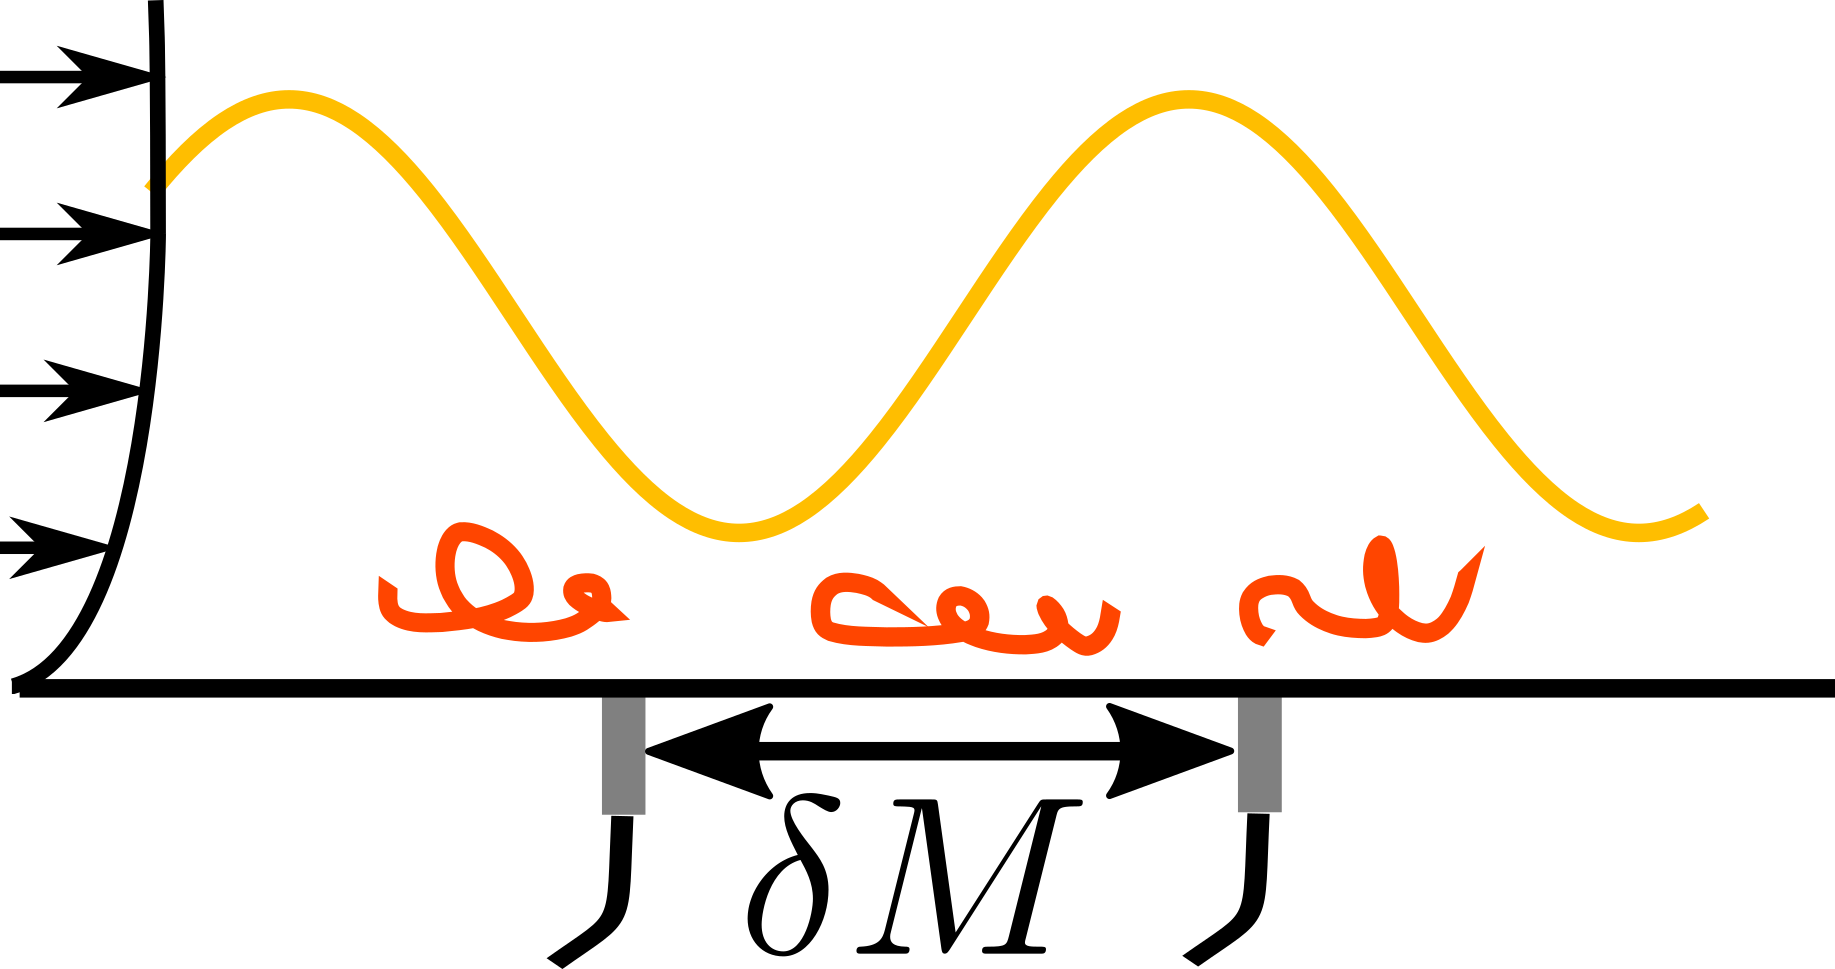
\includegraphics[width=1.1\textwidth]{idee.png}
\end{minipage}
\begin{minipage}{0.75\textwidth}
	\begin{itemize}
	        \item \textcolor{rouge}{bruit} faiblement corrélé \hfill\tikz[baseline]{\draw[->,>=latex] (0,0.5ex) -- ++(1.5em,0);} \textbf{MI diagonale~~~~~~}
	        \item \textcolor{jaune}{signal} acoustique corrélé \hfill\tikz[baseline]{\draw[->,>=latex] (0,0.5ex) -- ++(1.5em,0);}  \textbf{MI à rang réduit}\\  peu de monopoles équivalents 
	\end{itemize}
\end{minipage}\\[1em]
\onslide<2->{\tikz[baseline]{\draw[->,>=latex, line width=1.05pt] (0,1.3em) -- ++(0,-1.1em) -- ++(1.5em,0);} {\bfseries Faire une décomposition matricielle}\\[1em]}

\begin{overlayarea}{\textwidth}{0.3\textheight}
\centering
\includegraphics<3>[height=\textwidth,angle=-90]{model1.pdf}
\includegraphics<4>[height=\textwidth,angle=-90]{model2.pdf}
\includegraphics<5>[height=\textwidth,angle=-90]{model3.pdf}
\includegraphics<6>[height=\textwidth,angle=-90]{model4.pdf}
\includegraphics<7>[height=\textwidth,angle=-90]{model5.pdf}
\includegraphics<8>[height=\textwidth,angle=-90]{model6.pdf}
\includegraphics<9>[height=\textwidth,angle=-90]{model7.pdf}
\includegraphics<10>[height=\textwidth,angle=-90]{model8.pdf}
\end{overlayarea}

%\begin{minipage}{\textwidth}
%	\tikz[remember picture]{
%	\node[anchor=north west,color=black,text=black,inner sep=2pt, line width=1pt] (entrees) at  (current page.west) {\fbox{\parbox{0.4\textwidth}{\footnotesize Modèle de sources \\Modèle de bruit}} };\\
%	 \parbox{0.4\textwidth}{$\bm{M}(\theta_1,\theta_2,\dots,\theta_N)$\\ Chaque paramètre $\theta$}
%		\node[anchor=north] (gibbs) at (current page.center) {\includegraphics[width=0.5\textwidth]{00001.png}};		
%		\node[anchor=north east,shape=rectangle,color=black,text=black,inner sep=2pt, line width=1pt] (sorties)  at ($(current page.east)-(2cm,0)$) {\parbox{0.15\textwidth}{ \centering \bfseries \scriptsize
%		MI acoustique\\
%		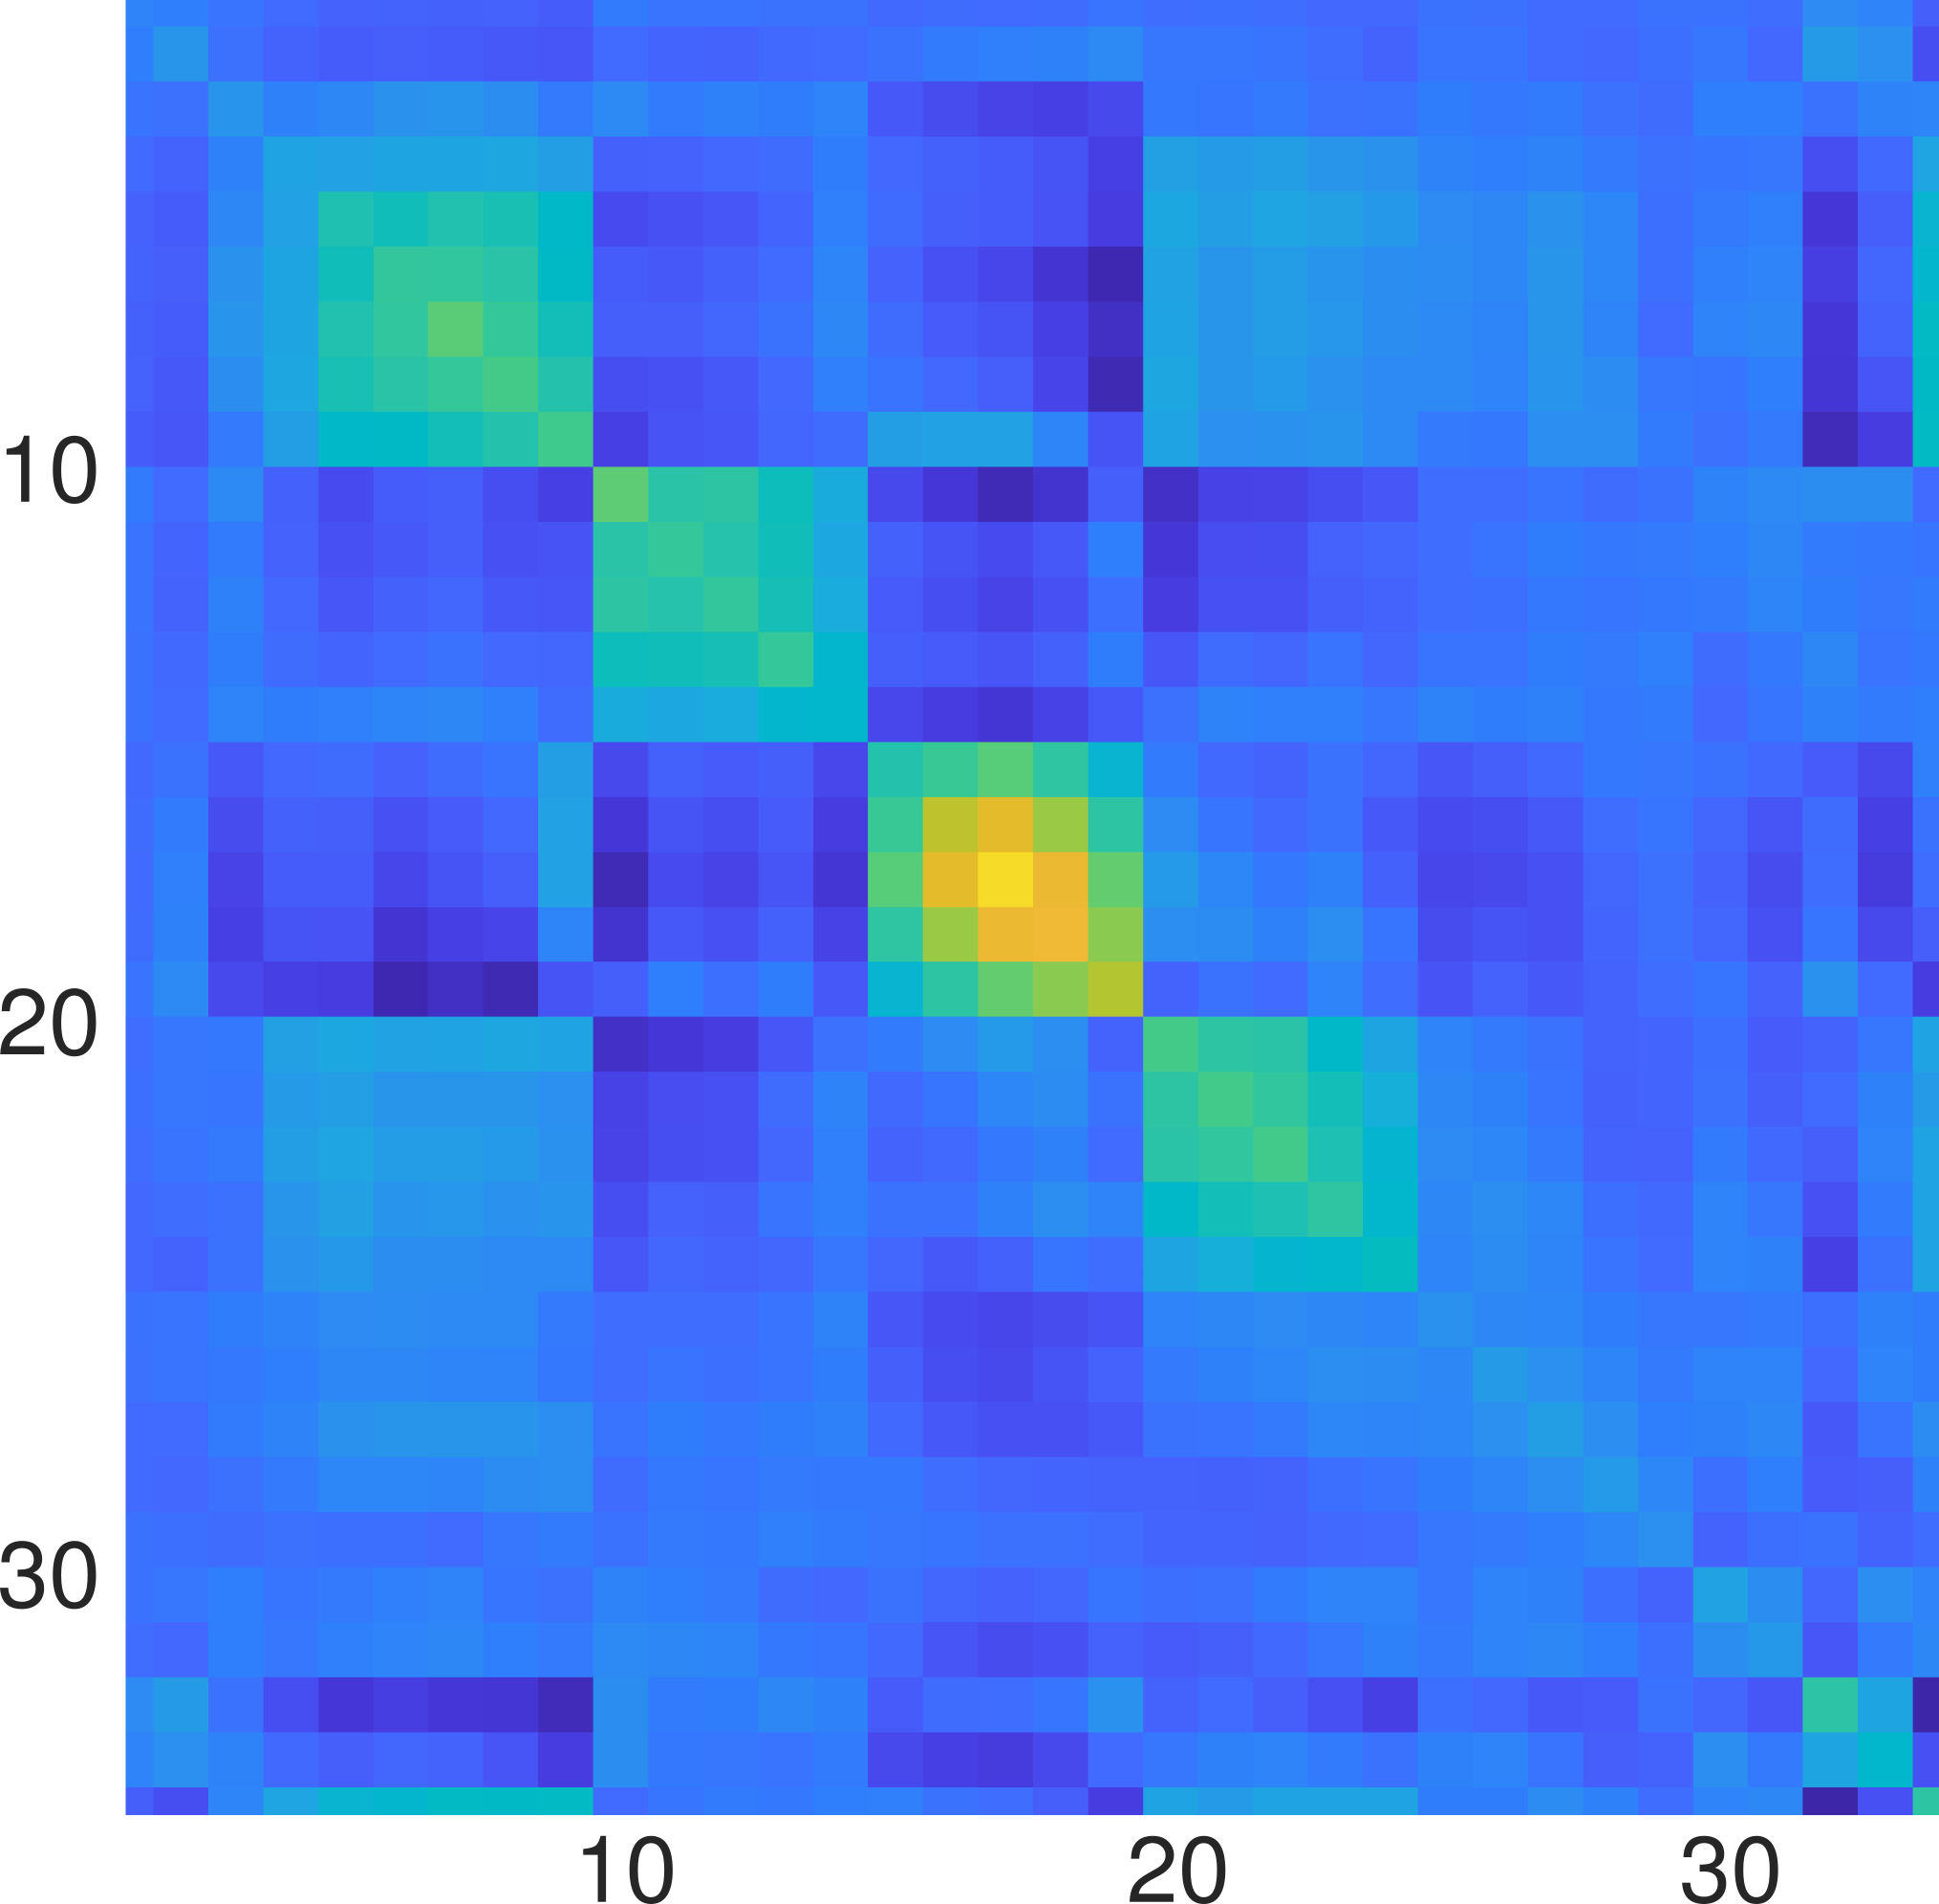
\includegraphics[width=\linewidth]{signal.png}\\
%		MI bruit\\
%		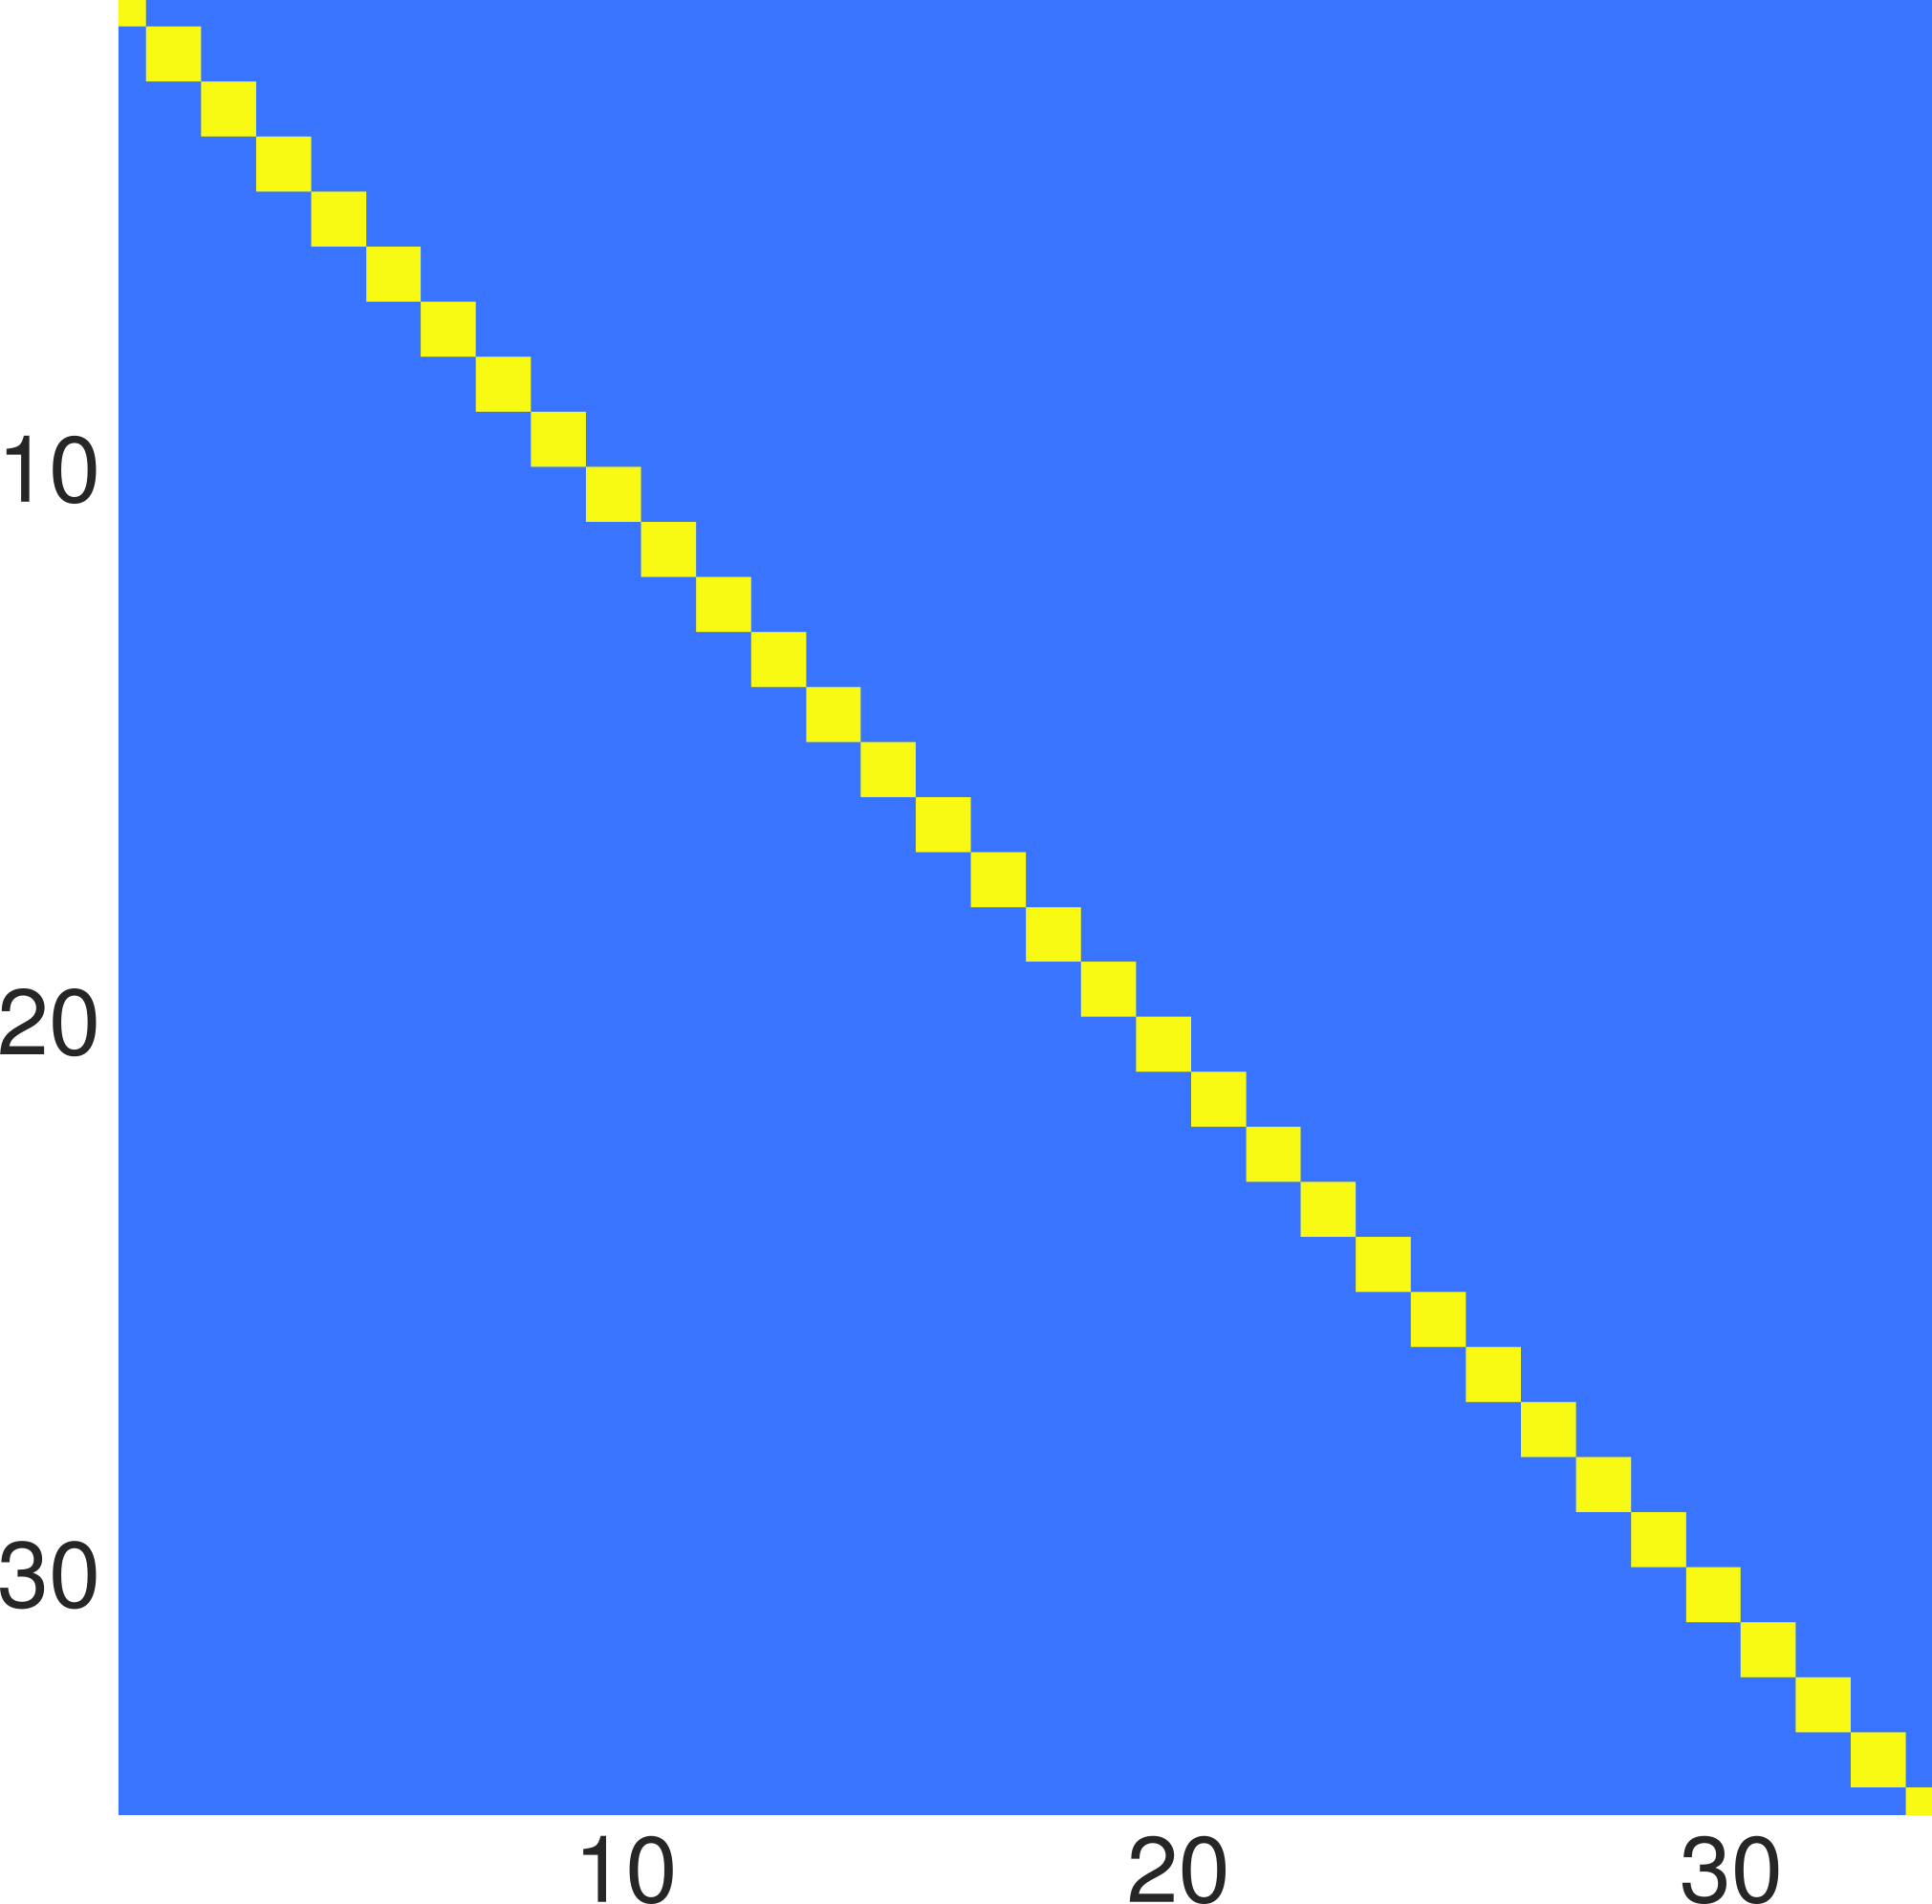
\includegraphics[width=\linewidth]{bruit.png}
%		}
%		};\hfill
%%	
%%		\draw[->,line width=1pt ,main,>=latex] (entrees) -- (gibbs);
%%
%}
%\end{minipage}

\end{frame}

%\section*{Méthode de débruitage}
%
%\begin{frame}{\insertsectionhead}
%	\begin{minipage}{0.2\textwidth}		
%		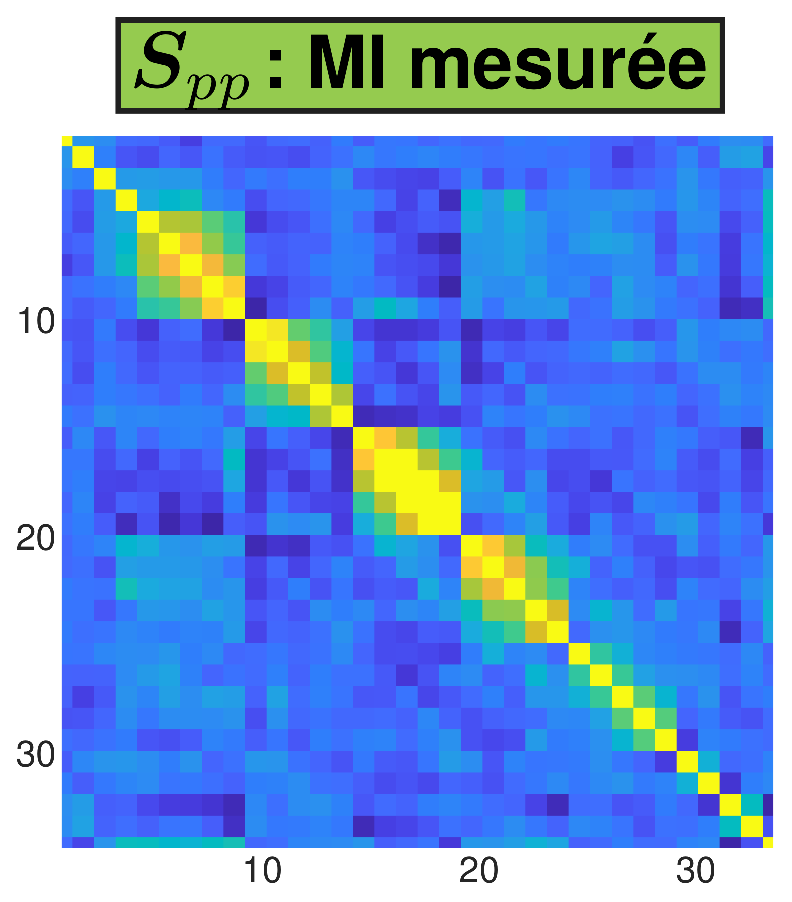
\includegraphics[width=1\textwidth]{csm.eps} \\[1ex]
%	\end{minipage}
%	\begin{minipage}{0.7\textwidth}
%		 \setlength{\tabcolsep}{0.7ex}
%		 \noindent \begin{tabular}{m{1.8ex} m{1ex} m{2\larg+\haut+2ex} m{1ex}  m{1.5\haut}}
%		%$\bm{S}_{pp~}$ & $=$ & \centering$\bm{L \diag{\alpha} S}_{cc} \bm{\diag{\alpha} L}'$&  $+$ &  \parbox{\linewidth}{ \centering $\diag{\bm{\sigma}^2_n}$} \\[1ex]
%			 & &  \parbox{\linewidth}{  \centering \small Matrice à rang réduit \\ $\overbrace{\hspace{\linewidth}}$} & & \parbox{\linewidth}{ \centering \small Bruit décorrélé \\ $\overbrace{\hspace{\linewidth}}$}\\
%		 & $=$  & \tikz{
%		 	\node at (0.5cm,0) (a) {};
%		 	\draw [rectangle,main,line width=1pt,fill=main!10] (a)  rectangle  ++ (\larg,-\haut)  ; 	 
%		 	\draw[rectangle,main,line width=1pt,fill=main!10] (a)++(\larg+0.1cm,-0.5\haut+0.5\larg) rectangle ++(\larg,-\larg);
%			\draw[main,rectangle,line width=1pt,fill=main!10] (a)++(2\larg+0.2cm,-0.5\haut+0.5\larg) rectangle ++(\haut,-\larg);
%			}
%			 & $+$ 
%			 &\begin{center}\tikz{
%			\draw[main,line width=1pt]  (0,0) rectangle ++(\haut,-\haut); 
%			\draw[line width=1pt,main] (0,0) to ++(\haut,-\haut);
%			}\end{center} \\
%			& & \centering 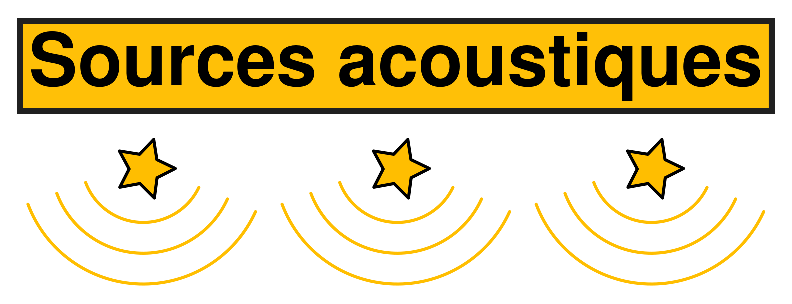
\includegraphics[scale=0.17]{sources.eps} && \centering 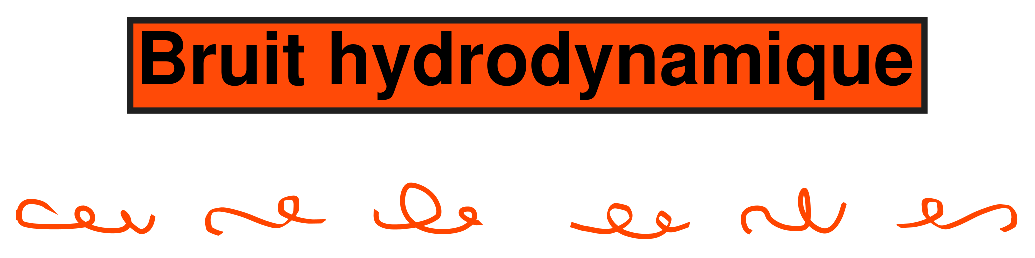
\includegraphics[scale=0.17]{bruit.eps}
%		\end{tabular}	
%		\vfill
%	\end{minipage}
%	
%\end{frame}

%\begin{frame}
%\tikz[remember picture,overlay]{
%	\node[anchor=center] (gibbs)  at (current page.center) {\includegraphics[width=0.3\textwidth]{00001.png}};
%	\node[anchor=west,shape=rectangle,color=main,text=black,draw,inner sep=2pt, line width=1pt] (donnees) {Mesures à débruiter};
%	\node[shape=rectangle,color=main,text=black,draw,inner sep=2pt, line width=1pt, below=of donnees] (param1) {Niveau du bruit};
%	\draw[->,line width=1pt ,main,>=latex] (donnees) -- (gibbs);
%	}
%\end{frame}
%\appendix
%%%% APPENDIX
%\setcounter{section}{0}
%\setbeamertemplate{headline}{%
%	\leavevmode%
%	\hbox{%
%		\begin{beamercolorbox}[wd=\paperwidth,ht=3ex,dp=1.125ex]{myheadline}%
%	   		\insertsectionnavigationhorizontal{\paperwidth}{}{}%
%	   	 \end{beamercolorbox}%
%	}
%}
%\newcounter{finalframe}
%\setcounter{finalframe}{\value{framenumber}}
%
%\section*{References}
%
%\begin{frame}{References}
%	%\begin{adjustwidth}{-2em}{-2.5em}
%		\setlength{\bibsep}{2em}
%		\bibliographystyle{abbrvnat}
%		\bibliography{biblio}
%	%\end{adjustwidth}
%\end{frame}
%
%
%
%\setcounter{framenumber}{\value{finalframe}}


%Texte du diapo \cite{Solomaa1973} et \cite{Dijkstra1982}
%\vfill
% 
%{\tiny 
%\usebibitemtemplate{\color{black}\insertbiblabel} 
%\usebibliographyblocktemplate{\color{black}}{\color{black}}{\color{black}}{\color{black}} 
% 
%\begin{thebibliography}{} 
%\bibitem{Solomaa1973} 
%A.~Salomaa. 
%\newblock {\em Formal Languages}. 
%\newblock Academic Press, 1973. 
%\bibitem{Dijkstra1982} 
%E.~Dijkstra. 
%\newblock Smoothsort, an alternative for sorting in situ. 
%\newblock {\em Science of Computer Programming}, 1(3):223--233, 1982. 
%\end{thebibliography} }


\end{document}